\documentclass{standalone}
\usepackage{tikz}
\usetikzlibrary{shapes,arrows,positioning}
\begin{document}
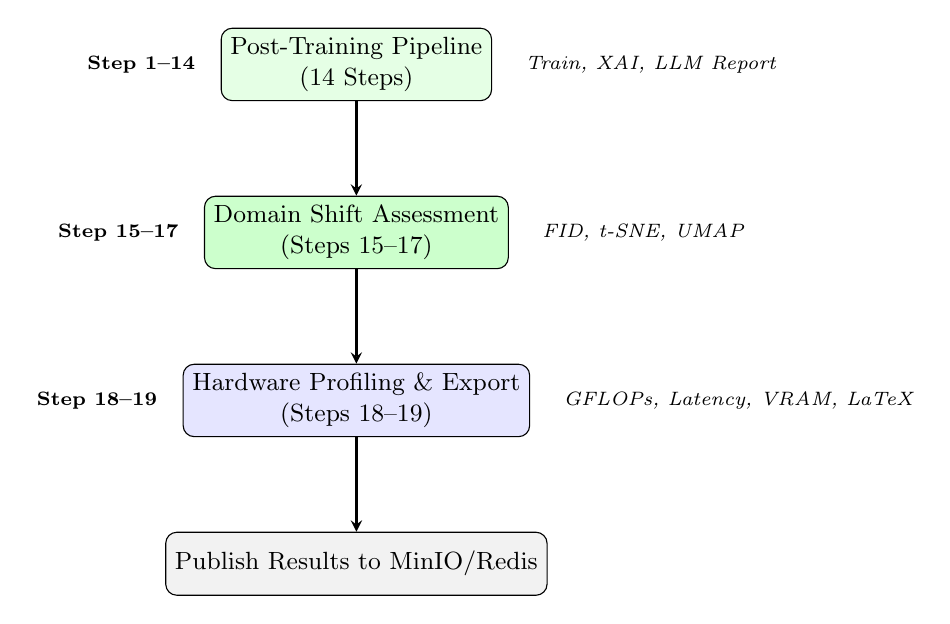
\begin{tikzpicture}[
    scale=0.9,
    every node/.style={font=\small},
    block/.style={draw, rounded corners, fill=#1, minimum width=3cm, minimum height=0.8cm, align=center},
    block/.default=green!10,
    arrow/.style={->, thick, >=stealth}
]
    % Pipeline block
    \node[block=green!10] (pipeline) {Post-Training Pipeline\\(14 Steps)};
    \node[right=0.3cm of pipeline, font=\scriptsize\itshape] {Train, XAI, LLM Report};

    % Domain Shift block
    \node[block=green!20, below=1.2cm of pipeline] (domain) {Domain Shift Assessment\\(Steps 15--17)};
    \node[right=0.3cm of domain, font=\scriptsize\itshape] {FID, t-SNE, UMAP};

    % Hardware block
    \node[block=blue!10, below=1.2cm of domain] (hardware) {Hardware Profiling \& Export\\(Steps 18--19)};
    \node[right=0.3cm of hardware, font=\scriptsize\itshape] {GFLOPs, Latency, VRAM, LaTeX};

    % Exit
    \node[block=gray!10, below=1.2cm of hardware] (exit) {Publish Results to MinIO/Redis};

    % Arrows
    \draw[arrow] (pipeline) -- (domain);
    \draw[arrow] (domain) -- (hardware);
    \draw[arrow] (hardware) -- (exit);

    % Labels
    \node[left=0.2cm of pipeline, font=\scriptsize] {\textbf{Step 1--14}};
    \node[left=0.2cm of domain, font=\scriptsize] {\textbf{Step 15--17}};
    \node[left=0.2cm of hardware, font=\scriptsize] {\textbf{Step 18--19}};
\end{tikzpicture}
\end{document}
